\documentclass[10pt]{exam}
\usepackage[phy]{template-for-exam}
\usepackage{tikz}
\usetikzlibrary{shadings,decorations.pathmorphing,arrows.meta,patterns}

\title{Momentum \#1}
\author{Rohrbach}
\date{\today}

\begin{document}
\maketitle

\begin{questions}
  
  \question
    A deer with a mass of 146 kg is running head-on toward you with a speed of 17 m/s. What is the momentum of the deer?
    \vs
  
  \question
    An 800-kg car is going 15 m/s before the engine applies a force of 750 N for 8 seconds.  What is the car's velocity now?
    \vs[2]

  \question
    A 12-kg hammer strikes a nail at a velocity of 8.3~m/s.  It comes to a rest in 0.012~seconds.  What is the average force that acts on the nail?
    \vs[2]

  \pagebreak

  \question
    A baseball is thrown by a pitcher with a velocity of 43 m/s. The batter hits {\bf straight back} at the pitcher with a velocity of 56 m/s. If the ball was in contact with the bat for 0.45 s, and has a mass of 0.145 kg, what is the force on the baseball? (\emph{Hint:} Be careful with your knowns and unknowns; one should be negative.)
    \vs
  
  \question
    A piece of putty and a bouncy ball, each of mass 0.035 kg, are thrown up against a wall. They each have an initial velocity of 5 m/s, but the bouncy ball returns towards the thrower with the same velocity, while the putty sticks to the wall. Which object has the larger change in momentum?

    \begin{center}
      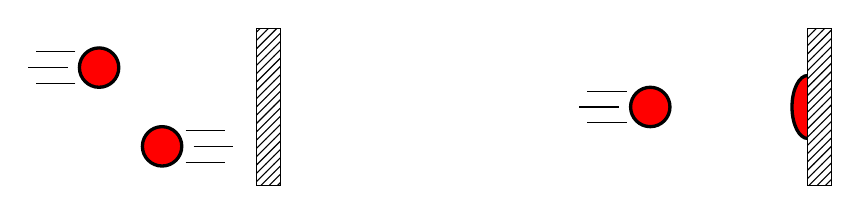
\begin{tikzpicture}
        \begin{scope}
          \draw[pattern=north east lines] (0,1) 
            rectangle (.3,-1);
          \draw[very thick,fill=red] (-2,0.5)
            coordinate (incoming) 
            circle (.25);
          \draw[thin] (incoming) ++ (-.3,.2) -- +(-.5,0);
          \draw[thin] (incoming) ++ (-.4,0) -- +(-.5,0);
          \draw[thin] (incoming) ++ (-.3,-.2) -- +(-.5,0);
          \draw[very thick,fill=red] (-1.2,-0.5)
            coordinate (outgoing)
            circle (.25);
          \draw[thin] (outgoing) ++ (.3,.2) -- +(.5,0);
          \draw[thin] (outgoing) ++ (.4,0) -- +(.5,0);
          \draw[thin] (outgoing) ++ (.3,-.2) -- +(.5,0);
        \end{scope}
  
        \begin{scope}[shift={(7,0)}]
  
          \draw[very thick,fill=red] (-2,0)
            coordinate (incoming) 
            circle (.25);
          \draw[thin] (incoming) ++ (-.3,.2) -- +(-.5,0);
          \draw[thin] (incoming) ++ (-.4,0) -- +(-.5,0);
          \draw[thin] (incoming) ++ (-.3,-.2) -- +(-.5,0);
          \draw[very thick,fill=red] (0,0)
            ellipse (.2 and .4);
          \fill[white] (0,1) 
            rectangle (.3,-1);
          \draw[pattern=north east lines] (0,1) 
            rectangle (.3,-1);
        \end{scope}
  
      \end{tikzpicture}
    \end{center}

    \vs
  
\end{questions}
\end{document}